\documentclass{beamer}
% Replace the \documentclass declaration above
% with the following two lines to typeset your 
% lecture notes as a handout:
%\documentclass{article}
\usepackage{CJKutf8}
\usepackage[T1]{fontenc}
%\usepackage[utf8x]{inputenc}
\usepackage{graphicx}
\usepackage{subfigure}
\usepackage{mathtools}
\usepackage{ulem}
\usepackage{url}
\usepackage{pifont}
\usepackage{pgfplots}
\usepackage{textcomp}

\usepgfplotslibrary{external}
\pgfplotsset{width=10cm,compat=1.9}

%% \usepackage{tikz}
%% \usepackage{verbatim}
%% \usepackage[active,tightpage]{preview}
%% \PreviewEnvironment{center}
%% \setlength\PreviewBorder{10pt}

\usetikzlibrary{shapes,arrows}

\tikzexternalize
\everymath{\displaystyle}

% There are many different themes available for Beamer. A comprehensive
% list with examples is given here:
% http://deic.uab.es/~iblanes/beamer_gallery/index_by_theme.html
% You can uncomment the themes below if you would like to use a different
% one:
%\usetheme{AnnArbor}
%\usetheme{Antibes}
%\usetheme{Bergen}
%\usetheme{Berkeley}
%\usetheme{Berlin}
%\usetheme{Boadilla}
%\usetheme{boxes}
%\usetheme{CambridgeUS}
%\usetheme{Copenhagen}
%\usetheme{Darmstadt}
%\usetheme{default}
%\usetheme{Frankfurt}
%\usetheme{Goettingen}
%\usetheme{Hannover}
%\usetheme{Ilmenau}
%\usetheme{JuanLesPins}
%\usetheme{Luebeck}
%\usetheme{Madrid}
%\usetheme{Malmoe}
%\usetheme{Marburg}
%\usetheme{Montpellier}
%\usetheme{PaloAlto}
%\usetheme{Pittsburgh}
%\usetheme{Rochester}
%\usetheme{Singapore}
%\usetheme{Szeged}
\usetheme{Warsaw}

%% \newcommand{chartnumproducts} {
%% }

\makeatletter
\pgfdeclareshape{datastore}{
  \inheritsavedanchors[from=rectangle]
  \inheritanchorborder[from=rectangle]
  \inheritanchor[from=rectangle]{center}
  \inheritanchor[from=rectangle]{base}
  \inheritanchor[from=rectangle]{north}
  \inheritanchor[from=rectangle]{north east}
  \inheritanchor[from=rectangle]{east}
  \inheritanchor[from=rectangle]{south east}
  \inheritanchor[from=rectangle]{south}
  \inheritanchor[from=rectangle]{south west}
  \inheritanchor[from=rectangle]{west}
  \inheritanchor[from=rectangle]{north west}
  \backgroundpath{
    %  store lower right in xa/ya and upper right in xb/yb
    \southwest \pgf@xa=\pgf@x \pgf@ya=\pgf@y
    \northeast \pgf@xb=\pgf@x \pgf@yb=\pgf@y
    \pgfpathmoveto{\pgfpoint{\pgf@xa}{\pgf@ya}}
    \pgfpathlineto{\pgfpoint{\pgf@xb}{\pgf@ya}}
    \pgfpathmoveto{\pgfpoint{\pgf@xa}{\pgf@yb}}
    \pgfpathlineto{\pgfpoint{\pgf@xb}{\pgf@yb}}
 }
}
\makeatother


\begin{document}

\newcommand{\plotNumProductChart} {
  \begin{tikzpicture}[scale=0.75]
    \begin{axis}[
        title={产品规模随时间的演变趋势},
        xlabel={年份},
        ylabel={度假搜索覆盖的单品数量(万)},
        xmin=2012, xmax=2015,
        ymin=0, ymax=120,
        xtick={2012,2013,2014,2015},
        ytick={0,20,40,60,80,100,120},
        legend pos=north west,
        ymajorgrids=true,
        grid style=dashed,
      ]
      
      \addplot[
        color=blue,
        mark=square,
      ]
      coordinates {
        (2012,10)(2013,29.5)(2014,59.5)(2015,108.4)
      };
      \legend{旅游度假产品数}
    \end{axis}
  \end{tikzpicture}
}

\newcommand{\plotGMVGrowthChart} {
  \begin{tikzpicture}[scale=0.75]
    \begin{axis}[
        title={GMV随时间的演变趋势},
        xlabel={年份},
        ylabel={日均GMV(万)},
        xmin=2012, xmax=2015,
        ymin=0, ymax=1200,
        xtick={2012,2013,2014,2015},
        ytick={0,200,400,600,800,1000,1200},
        legend pos=north west,
        ymajorgrids=true,
        grid style=dashed,
      ]
      
      \addplot[
        color=blue,
        mark=square,
      ]
      coordinates {
        (2012,25)(2013,130)(2014,500)(2015,950)
      };
      \legend{旅游度假事业部日均GMV}
    \end{axis}
  \end{tikzpicture}
}


\begin{CJK}{UTF8}{gbsn}

\title{度假搜索系统结构的演变}

% A subtitle is optional and this may be deleted
\subtitle{2015年Q4晋级答辩}

\author{李庚\inst{1}}
% - Give the names in the same order as the appear in the paper.
% - Use the \inst{?} command only if the authors have different
%   affiliation.

\institute[Qunar.com] % (optional, but mostly needed)
{
  \inst{1}
  旅游度假事业部-搜索及频道 \\
  Qunar.com
}
% - Use the \inst command only if there are several affiliations.
% - Keep it simple, no one is interested in your street address.

\date{\today}

\AtBeginSection[]
{
  \begin{frame}<beamer>{纲要}
    \tableofcontents[currentsection,currentsubsection]
  \end{frame}
}

\begin{frame}
  \titlepage
\end{frame}

\begin{frame}{自我介绍}
  \begin{columns}
    \column{0.4\textwidth}
    \begin{itemize}
      \item { 李庚 }
      \item { 2010年7月毕业,同年入职 }
    \end{itemize}
    \column{0.6\textwidth}
    \begin{itemize}[1]
      \item<2-> 度假搜索系统技术Leader
      \item<3-> QTalk Code Contributor, Emacs版QTalk开发者与维护者
    \end{itemize}
  \end{columns}  
\end{frame}

\begin{frame}{自我介绍(续)}
  \begin{itemize}
  \item {度假搜索系统技术Leader \& 产品需求规划}
  \end{itemize}
  \vspace{3 mm}
  \begin{columns}
    \column{0.6\textwidth}
    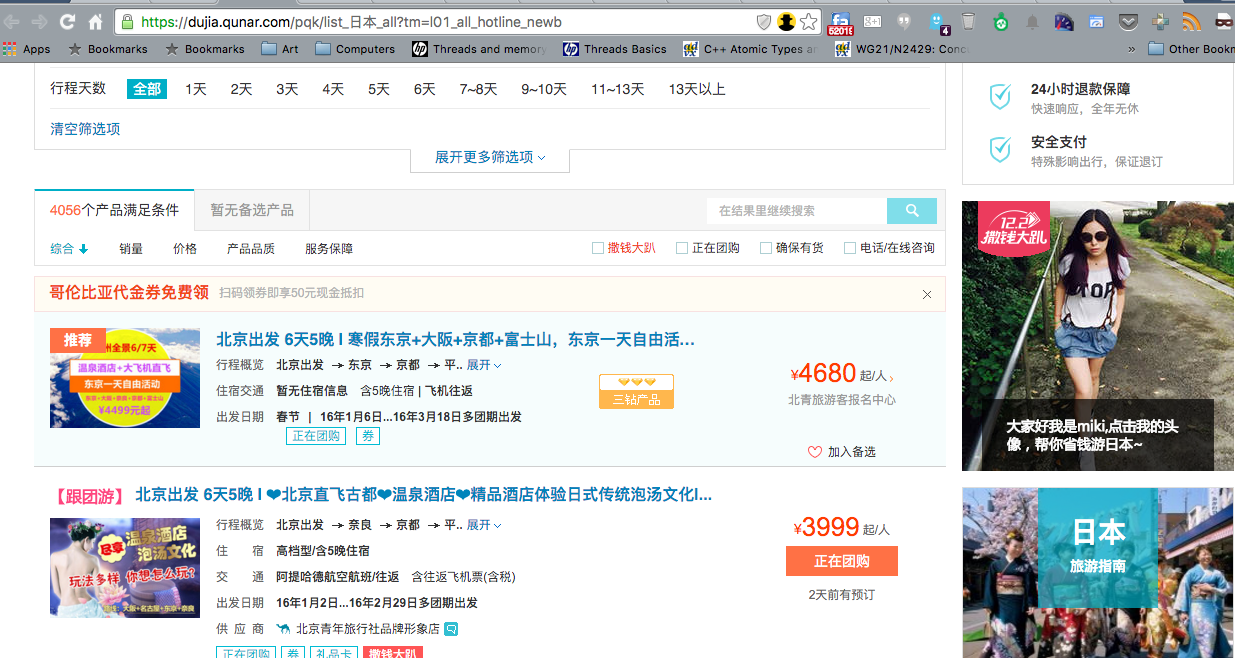
\includegraphics[scale=0.15]{./images/pc-search-screenshot}
    \column{0.4\textwidth}
    %% 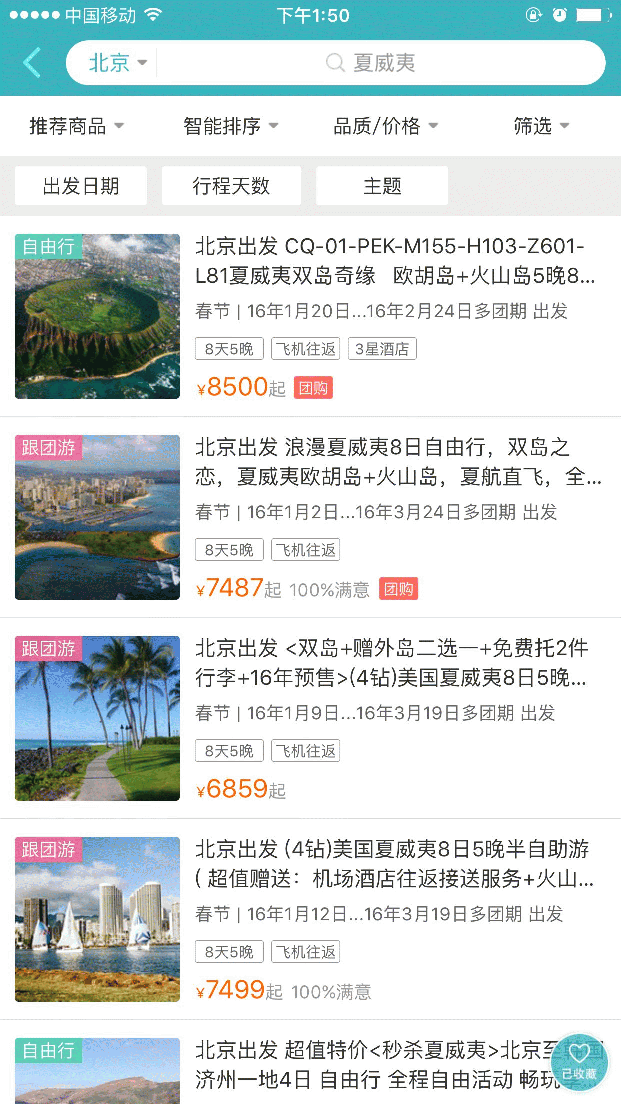
\includegraphics[scale=0.5]{./images/mobile-search-screenshot}
  \end{columns}
\end{frame}

\begin{frame}{自我介绍(续)}
  \begin{itemize}
  \item {QTalk Code Contributor, Emacs版QTalk开发者与维护者}
  \end{itemize}
  \begin{center}
    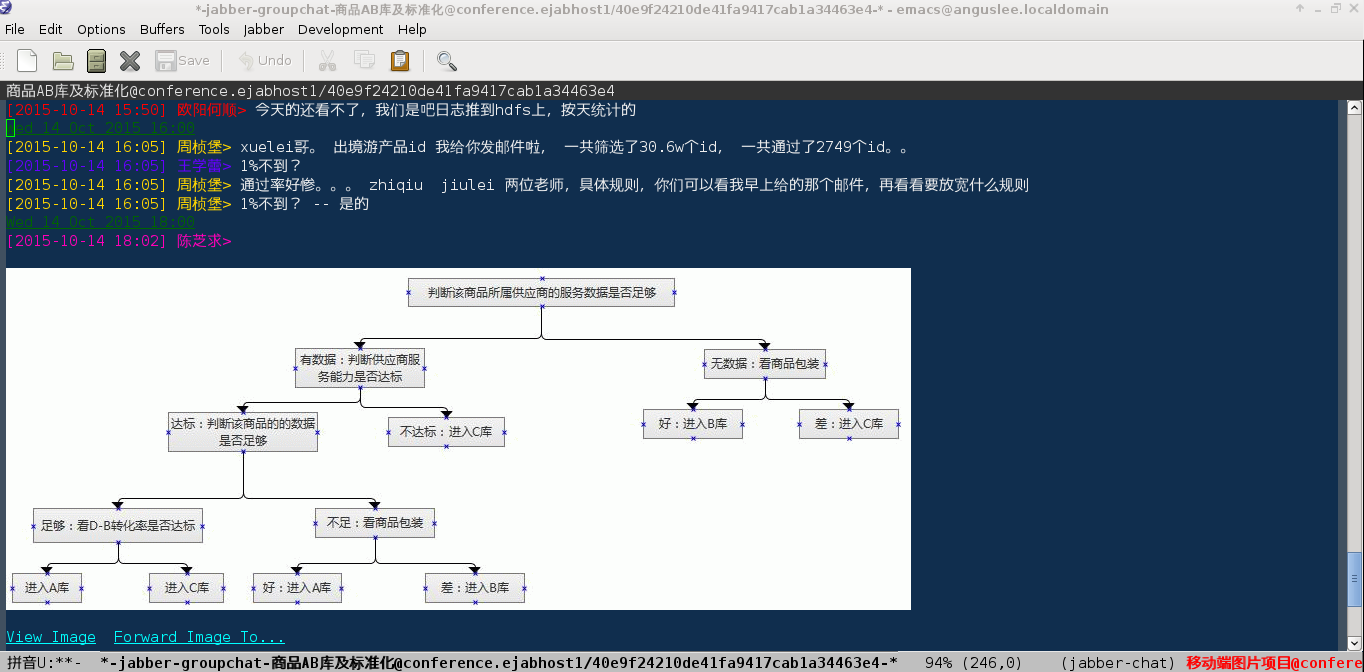
\includegraphics[scale=0.3]{./images/qtalk-emacs-screenshot}
  \end{center}
\end{frame}

\begin{frame}{纲要}
  \tableofcontents
\end{frame}

\section{搜索系统在业务中的定位}


\begin{frame}{事业部的目标}
  \begin{itemize}
  \item { 整合不同供应商提供的各类产品,满足用户的出行需求。
    \begin{itemize}
      \item<2-> { GMV: Gross Merchandise Value,总交易额 }
      \item<2-> { 毛利:$GMV - \text{成本} $ }
    \end{itemize}
  }
  \end{itemize}
\end{frame}

\begin{frame}{搜索团队要应对的问题}
  \begin{enumerate}
    \item { 随着业务量的膨胀,搜索服务的质量和效率不能降低 }
  \end{enumerate}
  \uncover<2-> {
    \begin{center}
      \plotGMVGrowthChart
    \end{center}
  }
\end{frame}


\begin{frame}{搜索服务的质量的量化定义}
  \begin{itemize}
  \item { $$ GMV = \sum_{i \in S}{(UV_i \times A_i \times R_i \times M_i)} $$ }
  \item { UV: 独立用户访问量 }
  \item { \color{blue}{ A: 服务可用率 } }
  \item { \color{blue}{ R: UV至订单转化率 } }
  \item { M: 平均用户交易额 }
  \item { S: 访问来源 }
  \end{itemize}
\end{frame}

\begin{frame}{搜索团队要应对的问题(续)}
  \begin{enumerate}\setcounter{enumi}{1}
  \item {
    应对不断变化的需求模式
    \begin{itemize}
      \item { 前期:PC为主 }
      \item { 目前:mobile为主 }
    \end{itemize}
  }
  \end{enumerate}
\end{frame}


\section{系统演变过程}

\begin{frame}{搜索系统技术结构}

  \begin{center}
    \begin{tikzpicture}[
        font=\sffamily,
        every matrix/.style={ampersand replacement=\&,column sep=1cm,row sep=.3cm},
        source/.style={draw,thick,rounded corners,fill=yellow!20,inner sep=.1cm},
        process/.style={draw,thick,circle,fill=blue!20},
        sink/.style={source,fill=green!20},
        datastore/.style={draw,very thick,shape=datastore,inner sep=.1cm},
        dots/.style={gray,scale=1},
        to/.style={->,>=stealth',shorten >=1pt,semithick,font=\sffamily\footnotesize},
        every node/.style={align=center}]

      % Position the nodes using a matrix layout
      \matrix{
        \node[source] (productsource) {旅游度假产品数据源}; \&
        \node[process] (searchengine) {搜索引擎}; \&
        \node[process] (webapi) {API接口}; \\

        \node[process] (crawling) {抓取打包}; \& 
        \node[datastore] (index) {倒排索引}; \&
        \node[process] (mining) {数据挖掘}; \\

        \node[datastore] (rawstorage) {产品原始数据}; \&
        \node[process] (preprocess) {预处理}; \&
        \node[datastore] (processedstorage) {服务数据}; \\
      };

      % Draw the arrows between the nodes and label them.
      %% \draw[to] (hisparcbox) -- node[midway,above] {raw events}
      %% node[midway,below] {level 0} (daq);
      %% \draw[to] (daq) -- node[midway,right] {raw event data\\level 1} (buffer);
      %% \draw[to] (buffer) --
      %% node[midway,right] {raw event data\\level 1} (monitor);
      %% \draw[to] (monitor) to[bend right=50] node[midway,above] {events}
      %% node[midway,below] {level 1} (storage);
      %% \draw[to] (storage) to[bend right=50] node[midway,above] {events}
      %% node[midway,below] {level 1} (monitor);
      %% \draw[to] (monitor) -- node[midway,above] {events}
      %% node[midway,below] {level 1} (datastore);
    \end{tikzpicture}
\end{center}
  
\end{frame}

\begin{frame}{搜索系统技术结构(续)}
  \begin{block}{对外服务端}
    \begin{itemize}
    \item { WEB与API }
    \item { 倒排索引 }
    \end{itemize}
  \end{block}
  \begin{block}{后台处理}
    \begin{itemize}
    \item { 数据预处理 }
    \item { 数据挖掘 }
    \end{itemize}
  \end{block}
\end{frame}

\begin{frame}{基本原则}
  \begin{enumerate}
  \item {
    量化目标
    \begin{itemize}
    \item<2-> { 产品需求:明确的量化指标和评测方法; }
    \item<2-> { 技术需求:制定监控目标,总结效果; }
    \end{itemize}
  }
  \item {
    重视系统结构的效率
    \begin{itemize}
    \item<3-> { 降低故障和线上bug出现的可能性,使得团队多数时间在处理重要且不紧急的工作; }
    \item<3-> { 总结合适的设计模式快速满足常见需求; }
    \end{itemize}
  }
  \item {
    测量结果,快速试错
  }
  \end{enumerate}
\end{frame}



\section{经验总结}

\begin{frame}{产品的目的地如何获取?}
  PlaceHolder
\end{frame}


\end{CJK}
\end{document}
